% The first command in your LaTeX source must be the \documentclass command.
\documentclass[sigconf]{acmart}
\usepackage{listings}
\usepackage{dirtytalk}
\usepackage[shortlabels]{enumitem}
\usepackage{amssymb}
\usepackage{minitoc}
\usepackage{algorithm}
\usepackage[noend]{algpseudocode}
\usepackage{mathtools}

% pseudocode
\algnewcommand\algorithmicforeach{\textbf{for each}}
\algdef{S}[FOR]{ForEach}[1]{\algorithmicforeach\ #1\ \algorithmicdo}

\DeclarePairedDelimiter{\ceil}{\lceil}{\rceil}


%
% \BibTeX command to typeset BibTeX logo in the docs
\AtBeginDocument{%
  \providecommand\BibTeX{{%
    \normalfont B\kern-0.5em{\scshape i\kern-0.25em b}\kern-0.8em\TeX}}}

% Rights management information. 
% This information is sent to you when you complete the rights form.
% These commands have SAMPLE values in them; it is your responsibility as an author to replace
% the commands and values with those provided to you when you complete the rights form.
%
% These commands are for a PROCEEDINGS abstract or paper.
\copyrightyear{2020}
\acmYear{2020}
\setcopyright{acmlicensed}
\acmConference[MileTS '20]{MileTS '20: 6th KDD Workshop on Mining and Learning from Time Series}{August 24th, 2020}{San Diego, California, USA}
\acmBooktitle{MileTS '20: 6th KDD Workshop on Mining and Learning from Time Series, August 24th, 2020, San Diego, Claifornia, USA}
\acmPrice{15.00}
\acmDOI{10.1145/1122445.1122456}
\acmISBN{978-1-4503-9999-9/18/06}

%
% These commands are for a JOURNAL article.
%\setcopyright{acmcopyright}
%\acmJournal{TOG}
%\acmYear{2018}\acmVolume{37}\acmNumber{4}\acmArticle{111}\acmMonth{8}
%\acmDOI{10.1145/1122445.1122456}

%
% Submission ID. 
% Use this when submitting an article to a sponsored event. You'll receive a unique submission ID from the organizers
% of the event, and this ID should be used as the parameter to this command.
%\acmSubmissionID{123-A56-BU3}

%
% The majority of ACM publications use numbered citations and references. If you are preparing content for an event
% sponsored by ACM SIGGRAPH, you must use the "author year" style of citations and references. Uncommenting
% the next command will enable that style.
%\citestyle{acmauthoryear}

%
% end of the preamble, start of the body of the document source.
\begin{document}

%
% The "title" command has an optional parameter, allowing the author to define a "short title" to be used in page headers.
\title{Lightweight Real-Time Feature Monitoring}

%
% The "author" command and its associated commands are used to define the authors and their affiliations.
% Of note is the shared affiliation of the first two authors, and the "authornote" and "authornotemark" commands
% used to denote shared contribution to the research.
\author[Conde]{João Conde}
\email{joao.conde@feedzai.com}
\affiliation{%
  \institution{Feedzai}
}

\author[Sampaio]{Marco O. P. Sampaio}
\email{marco.sampaio@feedzai.com}
\affiliation{%
  \institution{Feedzai}
}

\author[Cardoso]{Pedro Cardoso}
\email{pedro.cardoso@feedzai.com}
\affiliation{%
	\institution{Feedzai}
}

\author[Ribeiro]{Pedro Ribeiro}
\email{pribeiro@dcc.fc.up.pt}
\affiliation{%
  \institution{University of Porto}
}

\author[Restivo]{André Restivo}
\email{arestivo@fe.up.pt}
\affiliation{%
	\institution{University of Porto}
}
    


%
% By default, the full list of authors will be used in the page headers. Often, this list is too long, and will overlap
% other information printed in the page headers. This command allows the author to define a more concise list
% of authors' names for this purpose.
\renewcommand{\shortauthors}{Trovato and Tobin, et al.}

%
% The abstract is a short summary of the work to be presented in the article.
\begin{abstract}
Many real-time stream monitoring systems are static once deployed in a production environment. Over time, due to data pattern shifts, the initially deployed static system's performance gradually deteriorates. Data pattern shift detection refers to the process of finding patterns in data that do not conform to expected or usual behavior. Accurate and timely detection of data pattern deviations allow for immediate measures to be taken. Thus, the problem at hand is to determine when to reconfigure the system, \textit{e.g.}, a Machine Learning model, based on an analysis of the drifts in the stream of data. In this paper, we present a method that makes use of constant time & memory streaming aggregations and distribution divergence functions to alert deviations in data patterns in real-time. We generate alerts based on a user-defined probability threshold, for each of an event's fields, denominated features in our context. We evaluate our method through a series of tests, some with synthetic data sets and some with real data. We further split the tests into single and multi-feature analysis. Our method accurately detected the introduced anomalies in the experiments using synthetic datasets while maintaining high throughput, for single and multi-feature analysis. However, experiments with real data were not as accurate. Despite not knowing the specific reasons for that, we detail further investigation to future work and formulate a set of hypotheses that might explain the latter results and hence are worthy of pursuing next. Moreover, our set of experiments support the claim that sliding window aggregations and distribution divergence methods can be combined to detect data pattern shifts in streaming scenarios with constant time and memory complexity.
\end{abstract}

%
% The code below is generated by the tool at http://dl.acm.org/ccs.cfm.
% Please copy and paste the code instead of the example below.
%
\begin{CCSXML}
<ccs2012>
   <concept>
       <concept_id>10002951.10003227.10003351.10003446</concept_id>
       <concept_desc>Information systems~Data stream mining</concept_desc>
       <concept_significance>500</concept_significance>
       </concept>
   <concept>
       <concept_id>10010520.10010570.10010574</concept_id>
       <concept_desc>Computer systems organization~Real-time system architecture</concept_desc>
       <concept_significance>500</concept_significance>
       </concept>
 </ccs2012>
\end{CCSXML}

\ccsdesc[500]{Information systems~Data stream mining}
\ccsdesc[500]{Computer systems organization~Real-time system architecture}

%
% Keywords. The author(s) should pick words that accurately describe the work being
% presented. Separate the keywords with commas.
\keywords{data streams, monitoring, real-time, lightweight, concept drift}


%
% This command processes the author and affiliation and title information and builds
% the first part of the formatted document.
\maketitle

\section{Introduction}
In the past decade, applications have become increasingly data-driven, placing data at the center of application design. For different use cases, the data is processed in different ways for different purposes. For instance, e-commerce platforms such as Alibaba\footnote{https://alibaba.com} need to process a large number of daily transactions while ensuring that sales run smoothly and that products are delivered to customers' homes. Streaming services, like YouTube\footnote{https://youtube.com} and Netflix\footnote{https://netflix.com}, try to guarantee that media content reaches up to millions of users simultaneously. Social networks are responsible for generating large volumes of data. Twitter\footnote{https://twitter.com}, for example, generates more than 500 million \textit{tweets} (posts in Twitter) per day\footnote{https://blog.twitter.com/engineering/en\_us/a/2013/new-tweets-per-second-record-and-how.html}. \textit{Tweets} may contain text, media content or both. Cybersecurity applications are yet another example of time-sensitive, data-driven applications. The entities that work in these use cases need to monitor user accesses and their actions in the network, where timely detection of intruders is critical to prevent them from tampering with the underlying system.

All of these applications generate large volumes of data which lead to the creation of multiple real-time unbounded datasets, also known as data streams. The information that flows through such a stream can be analyzed on-the-fly or stored for later processing. The former is best known as stream processing, whereas the latter is known as batch processing. Streaming data is known for being non-stationary \cite{Gama-Knowledge-Discovery} where the value of the produced information lies in its recency \cite{Kolajo-Big-data-stream-SLR}. \textit{Recency} is measured under different scales for different use cases. For instance, consider the monitoring of geological data to forecast possible natural disasters such as earthquakes versus the monitoring of a computer network for intruder detection. In the former case, after the forecast of a future earthquake, governmental authorities need a couple of days to launch an evacuation plan and keep the population safe. However, in the intruder detection scenario, the decision of removing access to a user must be done as soon as possible, preferably in a few seconds. Hence, while in the first scenario information retrieved within a day would still be recent, in the second scenario, information is considered recent and relevant if delivered within seconds (or even milliseconds).

Consider the use case where we want to detect credit card fraud on the data stream of all the transactions made on Amazon\footnote{https://amazon.com} by every US citizen on a single day. In this case, Amazon's transaction stream will need to be monitored by another system, a fraud detection one. Such a system would have to process all incoming transactions and decide, in a fraction of a second, if a transaction is fraudulent or not. Unlike the fraud detection system, our system is not mission-critical. Hence, it must monitor the data stream looking for data pattern deviations in real-time but with a low memory footprint.

To summarize, in this paper we design a lightweight real-time system that monitors a stream of high volumes of high velocity, highly skewed and seasonal data and detects pattern shifts relative to a reference period. The motivation to detect data stream pattern deviations in real-time is to know when to reconfigure the mission-critical system (\textit{e.g.}, retrain the Machine Learning model) before its performance decays. We want to build a lightweight enough solution that can be integrated into existing workflows since having a real-time system monitoring other real-time systems consuming as many resources as the latter would be far too costly.

\section{Related Work}
\label{sec:RelatedWork}


\section{Method}
\label{sec:Method}
A data stream is a continuous collection of events, each timestamped and with multiple fields. In this paper, we refer to the event's fields as features. Our goal is to detect data pattern deviations for each feature in a streaming fashion. To that end, we devise a method that works with two windows and comprises two phases, a batch analysis phase and a stream analysis one. The batch analysis is performed on a static in time window which we call the reference window. The stream analysis is performed over a sliding window that groups data stream events. We aggregate the contents of the reference and sliding windows using an approximate histogram aggregation based on Exponential Moving Averages (EMAs) \cite{EMA-Everett2011, EMA-Hunter, EMA-MarcusB}. We then apply a statistical distribution divergence function to both aggregations to obtain a divergence value. In the batch phase, we build the distribution of these values so we can define a percentile threshold for newly measured divergence values.

\subsection{Batch Analysis Phase} \label{sec:batch-phase}
The goal of the batch phase is to build our reference aggregation for each feature and get to know the distribution of divergence or distance values. In other words, for each feature, we:
\begin{enumerate}
    \item Compute the reference histogram using all data in the reference period
    \item Compute the distribution of distances between the reference histogram and random samples of data
\end{enumerate}

This distribution of values can then later be compared to a given value of divergence for a single sample to find out how probable that value is to occur (if it is very low an alert may be raised).

\subsubsection*{Building the Reference Histogram for each Feature}

First, for each feature, we compute the reference histogram from the reference period dataset. This is an exact histogram aggregation. When building it we ensure the histogram has equal counts (or equal height) for all bins which often results in different sized bins. We make no assumption on the dataset distributions and hence use equal height histograms because they adjust better to wildly varying ones. Equal height means we have more bins covering very dense regions (regions with many data points) and fewer bins in lower density regions. 

\begin{figure}[!htb]
    \begin{center}
      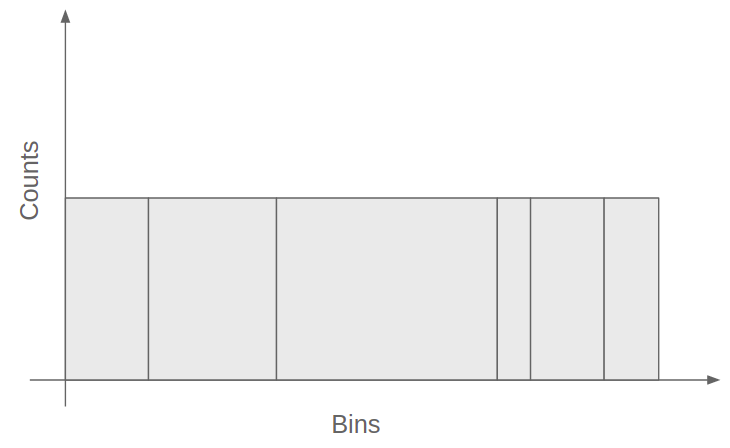
\includegraphics[scale=0.4]{figures/ref-hist.png}
      \caption[]{Reference equal-height histogram}
      \label{fig:ref-hist}
    \end{center}
\end{figure}


\subsubsection*{Finding the Distribution of Distances for each Feature} \label{sec:sampling-batch}

Secondly, we aim to build the histogram that encodes the distribution of expected distance values, to later on threshold the observed distance values during the online phase. To that end, we make $S$ samples of transactions (in Section \ref{sec:nsamples} we discuss the minimum number $S$ of samples to make), each with the same tuple-based size of the target sliding window we will use in streaming. Each sample is a contiguous block of transactions, thus preserving the order of transactions and the time-dependency property of a time-series. 

For each sample, and each feature, we compute the approximated histogram using the bins computed for the reference histogram (Figure \ref{fig:ref-hist-bins}). We also add two extra bins that will cover the region to the left and the right of our histogram, respectively. In other words, we add a bin that covers the region between $-\infty$ and our first bin and another that covers values from the last bin to $+\infty$. This way, observed values outside of the reference period will be placed in these special bins, either left or right.

\begin{figure}[!htb]
    \begin{center}
      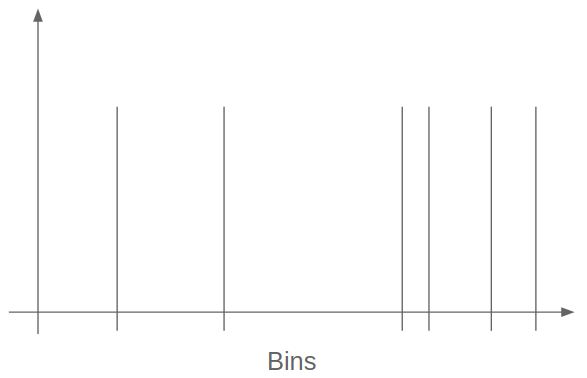
\includegraphics[scale=0.4]{figures/ref-bins.png}
      \caption[]{Reference equal-height histogram}
      \label{fig:ref-hist-bins}
    \end{center}
\end{figure}

Each of the histograms is an EMA-like histogram. An EMA-like histogram is essentially a collection of EMA-counts, as described in Section \ref{sec:ema-hist}. Each sample is processed event by event and a discount factor is applied per event to each bin (EMA expiration factor), thus building an approximated histogram aggregation, using the reference bins, for each feature of that sample. This procedure is illustrated in Figure \ref{fig:EMA-hist-build}.
\begin{figure}[!htb]
    \begin{center}
    \hspace{2cm}
      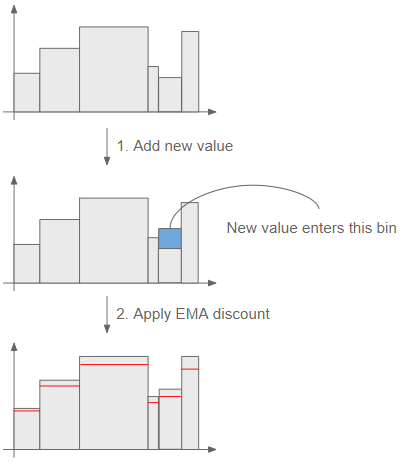
\includegraphics[scale=0.8]{figures/ema-hist.png}
      \caption[]{Reference equal-height histogram}
      \label{fig:EMA-hist-build}
    \end{center}
\end{figure}
We compute multiple sample histograms to encode distributions over smaller time periods that may exist within the large reference period. We use an approximated histogram to mimic the target approximated histogram we will incrementally maintain in the streaming environment.

For each feature, we have now \textit{S} histograms, one for each sample. For each of the \textit{S} histograms, we compute the distance between it and the reference histogram. Figure \ref{fig:compute-sample-distances} illustrates this process as we apply our distance function for each sample histogram and the reference histogram, obtaining \textit{S} distance measurements.

\begin{figure}[!htb]
    \begin{center}
      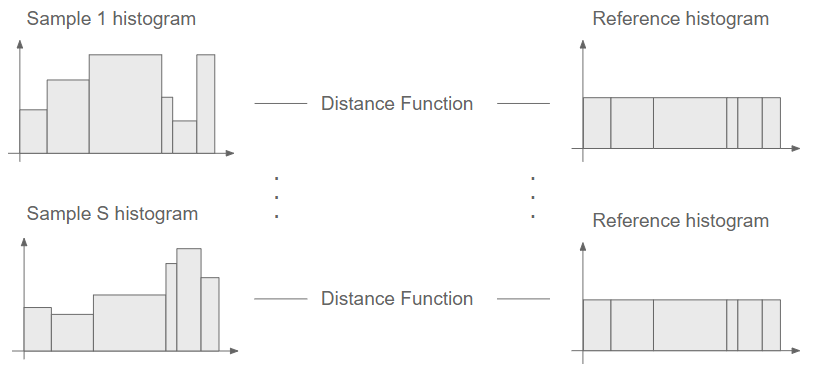
\includegraphics[scale=0.7]{figures/compute-sample-distances.png}
      \caption[Compute sample's distance values]{Compute as many distance values as samples, one for each sample-reference histogram pair}
      \label{fig:compute-sample-distances}
    \end{center}
\end{figure}

For each feature, we end up with \textit{S} distance values. These $S$ measurements are distance measurements between random samples of data and the reference period. Hence, we claim we now know the distribution of expected distance values. Given a new distance value measured between another random window and the reference window, we can compute its probability and produce alerts if the probability is below a certain threshold. Note that the histograms for each sample are EMA-like histograms (as detailed in Section \ref{sec:ema-hist}) just like the target sliding window histogram. This ensures a certain degree of fidelity in the test we make in streaming because we measure the divergence between a random sample of data (our streaming histogram or any of the sample's histogram) and the reference one.


It is important to understand why we want to know the distribution of divergence values instead of just thresholding the divergence value itself. For instance, given that JSD values vary between 0 and 1, why not just set to alert if the measured JSD value is 0.7? The reason is that a divergence value may fall on different percentiles for different features. In other words, the same \textit{i-th} percentile will correspond to a different divergence value for different features. Consider the following left and right-skewed distance distributions represented by Figures \ref{fig:skewed-left-distro} and \ref{fig:skewed-right-distro}, respectively. 

\begin{figure}[!htb]
    \begin{center}
      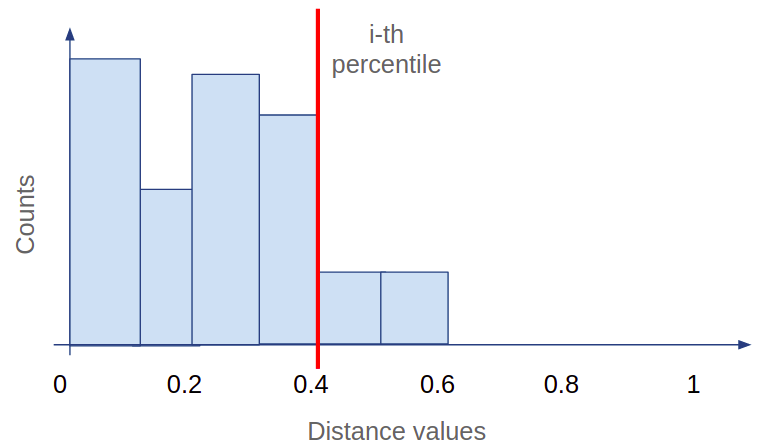
\includegraphics[scale=0.4]{figures/skewed-left-distro.png}
      \caption[]{Left skewed distribution of distance values}
      \label{fig:skewed-left-distro}
    \end{center}
\end{figure}

\begin{figure}[!htb]
    \begin{center}
      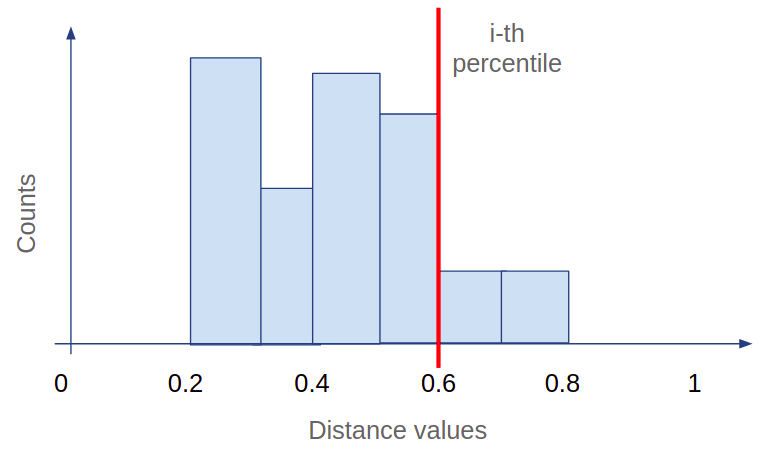
\includegraphics[scale=0.4]{figures/skewed-right-distro.png}
      \caption[]{Right skewed distribution of distance values}
      \label{fig:skewed-right-distro}
    \end{center}
\end{figure}

Let's assume that the histogram from Figure \ref{fig:skewed-left-distro} encodes the distribution of expected distance values for a feature \textit{x1} and Figure \ref{fig:skewed-right-distro} does the same but for a feature \textit{x2}. Setting a user-defined threshold of \textit{$\alpha$=0.6} for both features would yield very different results. For feature \textit{x1} we would be reporting distance values above the 100th-percentile which would not be the case for feature \textit{x2}. Instead, we define our threshold as a percentile of the distribution and not as a hard-coded distance constant. For instance, in this case, we would define the threshold to be the \textit{i}-th percentile, which would correspond to a threshold value of 0.4 for feature \textit{x1} and 0.6 for feature \textit{x2}.

Hard-coding a threshold value to be used for all features is cumbersome, impractical and error-prone. The distance threshold must be computed based on the distribution of distances.


\subsubsection*{Burn-In Period at System Initialization}
When we boot up our system in the streaming phase we initially have empty histogram aggregations. The period of time where you discard the alerts produced by the system until it processes enough data to produce accurate reports is commonly denoted as the burn-in period. To avoid this burn-in period we propose that the target sliding window approximate histogram aggregation for each feature is initialized using the last sample's histogram for that feature.

\subsubsection*{Batch Phase Artifacts} \label{sec:batch-artifacts-summary}
By the end of the batch phase, we should have, for each feature: 
\begin{itemize}
    \item a reference histogram
    \item a list of distance values that represent its distribution
    \item the last sample's histogram, to be used as burn-in period for the target sliding window histogram
\end{itemize}

\section{Experiments}
\label{sec:Experiments}

Much scientist

\section{Discussion}
\label{sec:Discussion}

Fight

\section{Conclusions}
\label{sec:Conclusions}
\cite{ApacheFlink}
Thesis done, PogU

\section{CCS Concepts and User-Defined Keywords}

Two elements of the ``acmart'' document class provide powerful taxonomic tools for you to help readers find your work in an online search. 

The ACM Computing Classification System --- \url{https://www.acm.org/publications/class-2012} --- is a set of classifiers and concepts that describe the computing discipline. Authors can select entries from this classification system, via \url{https://dl.acm.org/ccs/ccs.cfm}, and generate the commands to be included in the \LaTeX\ source. 

User-defined keywords are a comma-separated list of words and phrases of the authors' choosing, providing a more flexible way of describing the research being presented.

CCS concepts and user-defined keywords are required for all short- and full-length articles, and optional for two-page abstracts. 

\section{Tables}

The ``\verb|acmart|'' document class includes the ``\verb|booktabs|'' package --- \url{https://ctan.org/pkg/booktabs} --- for preparing high-quality tables. 

Table captions are placed {\it above} the table.

Because tables cannot be split across pages, the best placement for them is typically the top of the page nearest their initial cite.  To ensure this proper ``floating'' placement of tables, use the environment \textbf{table} to enclose the table's contents and the table caption.  The contents of the table itself must go in the \textbf{tabular} environment, to be aligned properly in rows and columns, with the desired horizontal and vertical rules.  Again, detailed instructions on \textbf{tabular} material are found in the \textit{\LaTeX\ User's Guide}.

Immediately following this sentence is the point at which Table~\ref{tab:freq} is included in the input file; compare the placement of the table here with the table in the printed output of this document.

\begin{table}
  \caption{Frequency of Special Characters}
  \label{tab:freq}
  \begin{tabular}{ccl}
    \toprule
    Non-English or Math&Frequency&Comments\\
    \midrule
    \O & 1 in 1,000& For Swedish names\\
    $\pi$ & 1 in 5& Common in math\\
    \$ & 4 in 5 & Used in business\\
    $\Psi^2_1$ & 1 in 40,000& Unexplained usage\\
  \bottomrule
\end{tabular}
\end{table}

To set a wider table, which takes up the whole width of the page's live area, use the environment \textbf{table*} to enclose the table's contents and the table caption.  As with a single-column table, this wide table will ``float'' to a location deemed more desirable. Immediately following this sentence is the point at which Table~\ref{tab:commands} is included in the input file; again, it is instructive to compare the placement of the table here with the table in the printed output of this document.

\begin{table*}
  \caption{Some Typical Commands}
  \label{tab:commands}
  \begin{tabular}{ccl}
    \toprule
    Command &A Number & Comments\\
    \midrule
    \texttt{{\char'134}author} & 100& Author \\
    \texttt{{\char'134}table}& 300 & For tables\\
    \texttt{{\char'134}table*}& 400& For wider tables\\
    \bottomrule
  \end{tabular}
\end{table*}

\section{Figures}

The ``\verb|figure|'' environment should be used for figures. One or more images can be placed within a figure. If your figure contains third-party material, you must clearly identify it as such, as shown in the example below.
\iffalse
\begin{figure}[h]
  \centering
  \includegraphics[width=\linewidth]{sample-franklin}
  \caption{1907 Franklin Model D roadster. Photograph by Harris \& Ewing, Inc. [Public domain], via Wikimedia Commons. (\url{https://goo.gl/VLCRBB}).}
  \Description{The 1907 Franklin Model D roadster.}
\end{figure}
\fi 
Your figures should contain a caption which describes the figure to the reader. Figure captions go below the figure. Your figures should {\bf also} include a description suitable for screen readers, to assist the visually-challenged to better understand your work.

Figure captions are placed {\it below} the figure.


\bibliographystyle{ACM-Reference-Format}
\bibliography{myrefs.bib}

\end{document}
